\documentclass[11pt,a4paper,spanish]{book}
%\usepackage{estilo_unir}
\usepackage{biblatex}
% Le dice a LateX desde donde incluir las imagenes
\usepackage{graphicx}
\graphicspath{ {./.images/} }
\usepackage{float}
\usepackage{hyperref}
\usepackage[utf8]{inputenc}
\addbibresource{./bibLib/mycol_arte.bib}

\begin{document}
	%---------------------------
	%título del trabajo y autor
	%---------------------------
	\title{Reconocimiento y clasificación de emociones en la lengua no aprendidas}
	\author{Luisa Sánchez Avivar}
	%\date{d de mes de 2019}
	%\director{CiroRodríguez}
	%\nombreciudad{Lausanne}
	
	%---------------------------
	%marges
	%---------------------------
	%\usepackage[margin=1.9cm]{geometry}
	%---------------------------
	%---------------------------
	%---------------------------
	%---------------------------
	\chapter{Estado del Arte}
	\section{Contexto}
	El reconocimiento de emociones en el habla es una disciplina en inteligencia artificial que trata de reconocer y clasificar emociones a través de la señal de voz. Este campo de estudio se ha hecho cada vez más popular, pero su origen se remonta a 1996, desde que se presentara el primer trabajo defendible sobre el tema "Reconociendo emociones en el habla" de la mano de F.Daellert \cite{Dellaert1996}.
	Desde entonces, el reconocimiento de emociones a través de la voz ha sido motivo de interés para la investigación, sin embargo en su gran mayoría, se ha estudiado sobre un mismo lenguaje debatiendo la habilidad de reconocer y clasificar las emociones oralmente expresadas. 
	
	\subsection{Temas fonéticos}
	El objetivo del reconocimiento de emociones en el habla es reconocer el trasfondo emocional del mensaje a través de la voz. Esta manifestación sonora posee factores clave para la comunicación humana que ayudan en su interacción sin alterar el contexto del mensaje.\\
	La expresión de las emociones están íntimamente relacionadas con las propiedades fonéticas en el habla donde se observan señales y patrones para marcar contrastes lingüísticos en un idioma \cite{Pell2001} por lo tanto, los efectos del lenguaje en la comunicación emocional son evidentes al haber sido observadas y medidas, las variaciones en el rango tonal y la frecuencia para expresarlas, cambiando no sólo el tono si no también el patrón lingüístico asociado \cite{Davletcharova2015}.
	Por otro lado tanto la proporción de consonantes y vocales (que hacen variar la presión de aire que se necesita) como el ratio de sílabas por palabra en cada idioma, caracterizan la expresión oral de las emociones. Existen muchos factores relacionados con el lenguaje como la morfología o la duración del estímulo que podrían ser un impacto en la decodificación de los matices en la señal vocal, tal y como se explica en \cite{Chen2017}.
	Existe una clasificación dependiendo de la velocidad silábica en la expresión de dichos idiomas, sin embargo poco se conoce acerca de los efectos en las medidas respiratorias en el habla. Esta observación puede llevar a que se pregunte si en lenguajes tan dispares, las emociones expresadas mediante la voz puedan ser reconocidas desde el punto de vista del otro idioma.
	Normalmente estos estudios se llevan a cabo en un único lenguaje, lo que en el caso que nos acontece, se traduciría como el reconocimiento de emociones llevado a cabo en la lengua materna; Mientras este ejercicio puede llegar a ser intuitivo, distinguir las mismas emociones en la lengua extranjera supone un reto ya que implicaría importantes matices culturales. Por ejemplo, no sería lo mismo entender qué emociones intenta expresar un italo parlante desde el punto de vista de una persona que entiende el español (ambas lenguas latinas), que comprender las mismas emociones del discurso desde un germano hablante. Así bien, es importante definir qué idioma se está reconociendo y desde cuál, por lo que analizar las raíces lingüísticas y fonéticas de los idiomas a estudiar es esencial. \hfill \break
	
	\subsection{Reconocimiento del habla}
	[...] Breve introducción a lo que se va a explicar
	
	\textbf{CLASIFICACIÓN DE EMOCIONES}
	De manera general, la clasificación de emociones se ha tratado desde dos enfoques principales:
	\begin{itemize}
		\item Las emociones como categorías discretas
		\item Las emociones vistas a través de un modelo dimensional
	\end{itemize}
	En el primer punto, a todos los humanos se les atribuye un conjunto de emociones básicas que pueden ser reconocidas interculturalmente. El debate se centra en la definición de dichas emociones, y fue Paul Elkman y su equipo en 1992 \cite{Ekman1992} quien estableció que estas eran 6: enfado, asco, miedo , felicidad, tristeza y sorpresa.
	En el segundo punto, las emociones se definen respecto a una o más dimensiones, donde normalmente las dimensiones que se comprenden tienden a ser la afectividad, la excitación o la intensidad. Aquí la discusión se centra en encontrar el número de dimensiones que de lugar a un modelo coherente y pueda incluir las emociones conocidas. El modelo de Plutchik \cite{Plutchik2001} sea quizá el más conocido en este enfoque, y propone un modelo tridimensional que organiza las emociones en círculos concéntricos situando la más básicas en el centro. \hfill \break
	
	\textbf{EXTRACCIÓN DE CARACTERÍSTICAS}
	La extracción de características es una de las secciones más importantes en el reconocimiento de emociones a través de la voz debido a la ambigüedad de las características y la variedad vocal. La extracción de características es el paso principal en el procesamiento del diálogo, y se lleva a cabo para centrarse en la información contenida en la señal y mejorar el grado de similitud y/o diferenciación entre las clases.\cite{Hellbernd2016} Hasta ahora, por lo general hay dos enfoques principales  con respecto al tipo de características usadas en el Reconocimiento de Emociones en el Discurso:\\
	Los rasgos prosódicos, los cuales extraen información de la prosodia, en concreto, tono, energía y duración, y por otro lado, las características del tracto vocal que normalmente indican la distribución de la energía en la frecuencia del rango vocal (conocidos como Coeficientes Cepstrales).
	La mayoría de los estudios centrados en este tema usan rasgos espectrales como la información extraída del tracto vocal, lo que supone obtener la información derivada del espectro de la señal de la voz y se usan para modelar los patrones de entonación y frecuencia del hablante\cite{Langari2020}.\\
	Comúnmente las técnicas de extracción de características más usadas son Coeficientes Cepstrales en la escala de Mel (MFCC), Coeficientes de Predicción Lineal (LPC), Coeficientes Cepstrales con Predicción Lineal (LPCC) y Transformada Wavelets Discreta (DWT).
	Tal y como se detalla en la revisión hecha por S.Rashid \cite{Rashid2018}, donde se ofrece una breve explicación de cada una de estas técnicas analizando sus puntos fuertes y débiles.\hfill \break 
	
	La \textbf{Transformada de Wavelets Discreta} descompone la señal en grupos de funciones básicas llamadas wavelets. La Transformada de Wavelet discreta es una extensión de esta donde mejora dicho proceso de descomposición discretizando los parámetros de tiempo y frecuencia. Los parámetros de DWT contienen información de diferentes escalas de frecuencia, lo cual es importante porque supone una mejora en la información que se obtiene del diálogo en la correspondiente banda de frecuencia. A pesar de ello, los coeficientes de Wavelet presentan variaciones indeseadas en los límites ya que las señales de entrada son de una longitud finita.\hfill \break
	
	Los \textbf{Coeficientes Cepstrales con Predicción Lineal} se aplican para obtener el coeficiente de predicción lineal equivalente al tracto vocal reduciendo el mínimo error cuadrado entre la señal de audio de entrada y la que es estimada. Normalmente se usa para extraer las propiedades del tracto vocal ya que hace estimaciones bastante precisas de los parámetros en el habla, no obstante, es altamente sensible al ruido de cuantificación, por lo que demuestra no ser precisa cuando hay ruido de fondo y podría, y al igual que MFCC, no ser apropiada para la generalización.\hfill \break
	
	Los \textbf{Coeficientes de Predicción Lineal} calcula una envolvente a LPC y luego hace una conversión a coeficientes cepstrales; Tiene una baja vulnerabilidad al ruido de fondo y mejora el ratio de error en comparación a LPC, pero sigue teniendo una gran sensibilidad al ruido de cuantificación.\hfill \break
	
	Los \textbf{Coeficientes Cepstrales en la escala de Mel}, se basan en la desintegración de la señal para tener como resultado un resumen de las características que la forman. La obtención de este conjunto de valores numéricos se basa por un lado, en el rango de frecuencias de Mel, el cual consiste en una adaptación de frecuencias de la señal a aquellas más fácilmente percibidas por el oído humano, y por lo otro lado, la separación de frecuencias mediante \emph{Cepstrum} que divide la señal en dos bandas de frecuencias, baja (correspondientes a los fonemas producidos por el tracto vocal) y alta (correspondientes a la excitación de las cuerdas vocales). Debido a esto, encapsula la mayor parte de energía proveniente del sonido que es generado por humanos, por lo que es frecuentemente usada y sugerida para identificar palabras monosilábicas en un discurso.
	
	Los objetivos clave, serían:
	\begin{itemize}
		\item Eliminar la excitación del tracto vocal.
		\item Hacer independientes a las características extraídas.
		\item Ajuste a como los humanos percibimos el ruido y la frecuencia del sonido.
		\item Capturar la dinámica fonética, que definirá el contexto.
	\end{itemize}
	
	\begin{figure}[H]
		\centering
		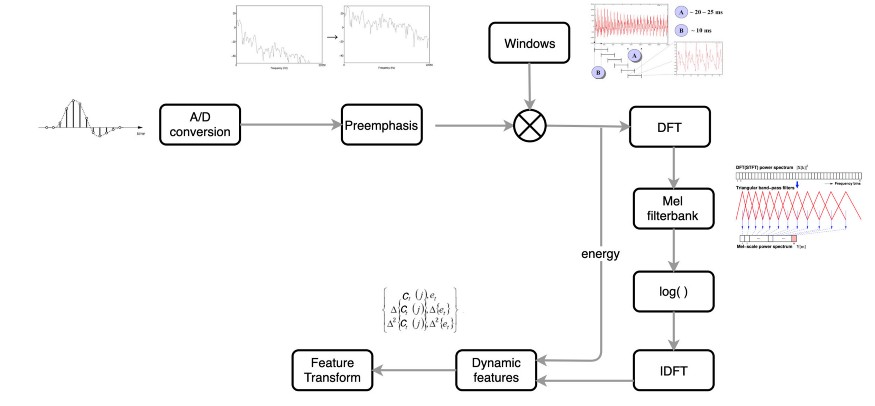
\includegraphics[scale=0.25]{MFCC_process.jpeg} 
		\caption{Proceso en la aplicación de MFCC en una señal.}
		\label{fig:mfcc_process}
	\end{figure}
	[...]
	
	Convencionalmente, el estudio de SER incluye el uso de diferentes tipos de clasificadores para distinguir entre emociones: Suport Vector Machines (SVNs) los cuales se han usado extensamente para el reconocimiento de emociones y pueden llegar a presentar un buen rendimiento en comparación con otros clasificadores tradicionales, el algoritmo K-NN es de los enfoques más simples, Hidden Markov Model(HMM) es a menudo utilizado para lidiar con los cambios temporales en la señal y por último, Gaussian Mixture Model (GMM) el cual es útil para representar las unidades de sonido en características acústicas \cite{Farooq2020}.
	No obstante,en estudios más recientes, se han propuesto clasificadores basados en aprendizaje profundo y en redes neuronales densas (DNN) los cuales han superado a los enfoques tradicionales resultando ser más eficientes además de tener la capacidad de aprender las características emocionales en el reconocimiento de emociones a través del audio.
	
	Las \textbf{Redes Recurrentes Neuronales} (RNN) son convenientes en tareas en las que los datos son procesados secuencialmente. 
	
	Los retos que presenta la clasificación de emociones en el habla, son comúnmente abordados a través de una red de \textbf{Memoria a Largo Corto-Plazo} (LSTM) la cual es capaz de retener información de entradas anteriores en el tiempo y tener en cuenta dependencias temporales largas, ya que cada nodo es una célula de memoria. Esto a su vez, resuelve el problema de desvanecimiento de gradientes que presenta RNN.
	
	La tendencia de los modelos basados en redes neuronales densas en este ámbito, es aprender características específicas desde varios métodos usados en el reconocimiento de emociones a través de la percepción acústica, en especial las \textbf{Redes Neuronales Convolucionales} (CNN) suponen una importante contribución en la clasificación emocional de la voz debido al uso de características significativas, y su uso en recientes estudios se ha incrementado a lo largo de los años.
	
	\section{Estado del Arte}
	
	En \cite{Harar2017} describe un método que utiliza una arquitectura basada en redes convolucionales sin selección de características para distinguir únicamente entre tres emociones en alemán (usando Berlin Database Emotional Speech, la cual contiene 800 muestras de audio etiquetadas) consiguiendo una exactitud de 96.97\%.
	
	En \cite{AbdulQayyum2019} se presenta un modelo de redes convolucionales que no necesita de un preprocesado de la señal para una clasificación de emociones en el idioma inglés. Este utiliza la base de datos SAVEE, la cual contiene 480 muestras que distinguen entre 6 emociones, interpretadas por hombres y mujeres angloparlantes, donde obtiene finalmente un 81.63\% de precisión.
	
	En el trabajo citado anteriormente \cite{Wang2020}, Wang propone un modelo dual LSTM para procesar dos espectogramas Mel simultáneamente, consiguiendo una precisión del 73.3\%. 
	Sin embargo este tipo de modelos no suelen implementarse como enfoque único, si no combinados con otro clasificador en una arquitectura más compleja.
	
	Por ejemplo en \cite{Lim2017} se lleva a cabo una comparación de tres  arquitecturas (CNN, LSTM y CNN distribuida en el tiempo) donde LSTM (utilizada de manera aislada) es la que puntúa más bajo.
	
	Por otro lado, W.Lim \cite{Lim2017} estudia el resultado de un sistema híbrido que usa CNN y RNN para clasificar emociones en una secuencia de audio, consiguiendo un 88.01\% de precisión.
	
	\section{Conclusiones parciales}
	En \cite{Langari2020} denota que los métodos de extracción de características son MFCC y LPCC porque las variaciones en la frecuencia del tono están significativamente relacionados con la expresión de emociones.
	
	
		
	\printbibliography
	
\end{document}